\section{Methods}\label{art.meth}
Here we describe the model parameterization and calibration,
followed by analyses for Objectives \ref{obj:art.1}~and~\ref{obj:art.2}.
\paragraph{Data Sources}
To inform our model, we used:
published aggregate data from four national surveys
in 2006--2021 \cite{SDHS2006,SHIMS1,SHIMS2,SHIMS3};
aggregate data from a 2021 FSW bio-behavioural survey \cite{EswIBBS2022}; and
individual-level data from two FSW bio-behavioural surveys
in 2011 \cite{Baral2014} and 2014 \cite{EswKP2014},
which were accessed under approval from
\blind{the Scientific and Ethics Committee of the Eswatini Ministry of Health (MH/599B)}, and
\blind{the Institutional Review Board of the Johns Hopkins Bloomberg School of Public Health (3508)}.
%===================================================================================================
\subsection{Model Parameterization \& Calibration}\label{art.meth.par}
The modelled population is stratified by
HIV status, sex, sexual activity, and the ART cascade of care.
Complete details of the model structure, parameterization, and calibration
are given in Appendix~\ref{mod}.
\mf{\begin{figure}
  \begin{subfigure}{\linewidth}
    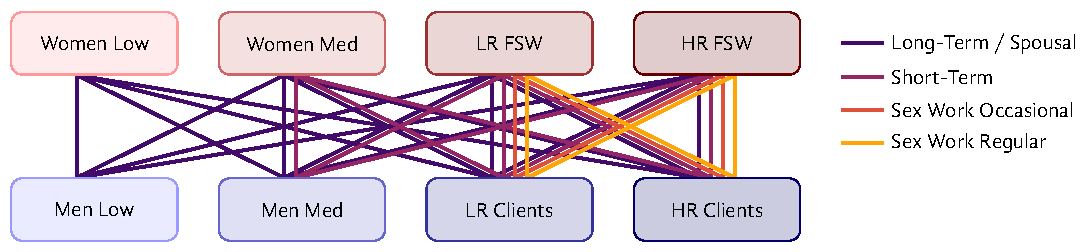
\includegraphics[scale=.8]{model.risk}
    \caption{Activity groups and partnership types}
    \label{fig:model.risk\mfx}
  \end{subfigure}
  \begin{subfigure}{\linewidth}
    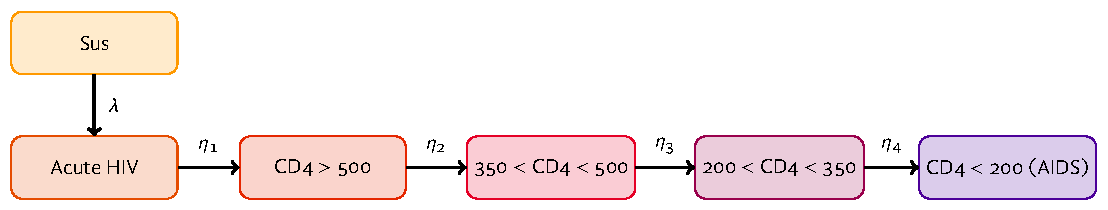
\includegraphics[scale=.8]{model.hiv}
    \caption{HIV states}
    \label{fig:model.hiv\mfx}
  \end{subfigure}
  \begin{subfigure}{\linewidth}
    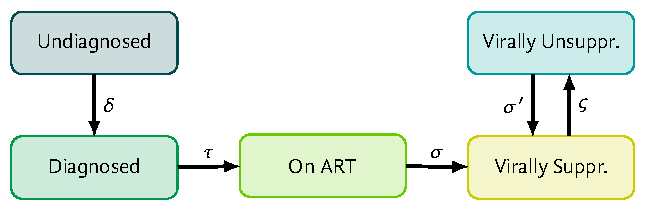
\includegraphics[scale=.8]{model.cascade}
    \caption{ART cascade states}
    \label{fig:model.cascade\mfx}
  \end{subfigure}
  \caption{Model structure and transitions}
  \label{fig:model\mfx}
  \floatfoot{
    \ffpops;
    CD4: CD4+ T-cell count per mm\tsup{3};
    ART: antiretroviral therapy;
    rates ---
    $\lambda$: force of infection;
    $\eta$: HIV progression;
    $\delta$: diagnosis;
    $\tau$: ART initiation;
    $\sigma$: viral suppression;
    $\sigma'$: viral re-suppression;
    $\varsigma$: ART failure / discontinuation;
    not shown: turnover amongst activity groups in \sfref{fig:model.risk}.}
\end{figure}
} % model figure
%---------------------------------------------------------------------------------------------------
\paragraph{HIV}
Modelled HIV natural history
includes acute infection and four stages defined by CD4-count:
\cdf{500}{}, \cdf{350}{500}, \cdf{200}{350}, and \cdf{}{200}
(Figure~\ref{fig:model.hiv.m}).
We modelled relative rates of infectiousness by stage
as an approximation of viral load \cite{Boily2009,Donnell2010,Bellan2015},
as well as rates of HIV-attributable mortality by stage \cite{Mangal2017}.
%---------------------------------------------------------------------------------------------------
\paragraph{Risk Heterogeneity}
The model includes eight subpopulations:
FSW and their clients at higher \vs lower risk,
plus other women and men with low and medium sexual activity
(0--1 and 2+ sexual partners in the past year, respectively);
and four sexual partnership types:
main/spousal, casual, repeat sex work, and one-off sex work
(Figure~\ref{fig:model.risk.m}).
We captured risk heterogeneity through:
subpopulation sizes, turnover among subpopulations, genital ulcer disease (GUD),
partnership formation rates and durations, preferential mixing, sex frequency, and condom use
(Table~\ref{tab:art.het}).
To parameterize FSW at higher \vs lower risk, we analyzed individual-level data
from Swati FSW in 2011 \cite{Baral2014} and 2014 \cite{EswKP2014}
(Appendix~\ref{mod.par.fsw}).
We parameterized the remaining subpopulations using data from
national surveys in 2006--2021 \cite{SDHS2006,SHIMS1,SHIMS2,SHIMS3}
(Appendix~\ref{mod.par.wp}--\ref{mod.par.pdur}).
We modelled
increasing condom use (Figure~\ref{fig:fit.condom}),
increasing voluntary medical male circumcision (Figure~\ref{fig:fit.circum}), and
decreasing GUD prevalence over time.
We did not model non-heterosexual HIV transmission
nor pre-exposure prophylaxis (PrEP),
which first became available in Eswatini in 2017
and reached 12\% of FSW by 2021 \cite{EswIBBS2022}.
\begin{table}
  \centering
  \caption{Selected model parameters related to risk heterogeneity}
  \footnotesize
% TODO: update
\begin{tabular}{llrclc}
  \toprule
                          &                                &  \multicolumn{3}{c}{Prior}   &         \\
  \cmidrule(rl){3-5}
  Parameter               & Stratification                 & Mean & (95\% CI)  & Distrib. &  Ref. * \\
  \midrule
  Population size         & FSW of women overall           &  2.8 & (0.6,~6.5) & Beta     &         \\
  (\% of total)           & Clients of men overall         &   30 & (6.0,~70)  & ---      & See~XX  \\
                          & HR FSW of FSW overall          &   20 &    ---     & ---      & Assumed \\
                          & HR clients of clients overall  &   20 &    ---     & ---      & Assumed \\[1ex]
  Duration in group       & HR FSW                         &  3.6 & (1.9,~5.8) & Gamma    & See~XX  \\
  (mean years)            & LR FSW                         &   10 & (9.0,~11)  & Gamma    & See~XX  \\
                          & All clients                    &   10 & (6.0,~15)  & Gamma    &         \\[1ex]
  Relative infectiousness & Acute infection                &  5.3 & (1.0,~13)  & Gamma    &         \\
                          & Any GUD p12m                   &  2.9 & (1.0,~5.7) & Gamma    &         \\[1ex]
  Relative susceptibility & Receptive vaginal sex          & 1.45 & (1.0,~2.0) & Gamma    &         \\
                          & Receptive anal sex             &   10 &    ---     & ---      &         \\
                          & Any GUD p12m: women            &  5.3 & (1.5,~12)  & Gamma    &         \\
                          & Any GUD p12m: men              &  7.7 & (2.0,~18)  & Gamma    &         \\[1ex]
  Any GUD p12m            & LR FSW                         &   16 &  (7,~28)   & Beta     &         \\
  prevalence (\%)         & HR FSW                         &   47 &  (19,~89)  & ---      &         \\
                          & HR clients                     &   12 &  (7,~22)   & ---      &         \\
                          & Everybody else                 &    7 &    ---     & ---      &         \\[1ex]
  Sex acts per            & Main/spousal                   &   78 & (27,~156)  & Gamma    &         \\
  partnership-year        & Casual                         &   30 & (4.4,~82)  & ---      & See~XX  \\
                          & Occasional sex work            &   12 &    ---     & ---      & Assumed \\
                          & Regular sex work               &   31 &  (18,~48)  & Gamma    &         \\[1ex]
  Partnership anal sex    & Main/spousal \& casual         &  5.9 & (0.6,~17)  & Beta     &         \\
  (\% of acts)            & Occasional \& regular sex work &  9.7 & (0.6,~29)  & Beta     &         \\[1ex]
  Condom use in 2020      & Main/spousal                   &   42 &  (31,~54)  & Beta     & See~XX  \\
  (\% of acts protected)  & Casual                         &   69 &  (65,~74)  & Beta     & See~XX  \\
                          & Occasional sex work            &   88 &  (78,~97)  & Beta     & See~XX  \\
                          & Regular sex work               &   79 &  (64,~90)  & Beta     & See~XX  \\
                          & Anal vs vaginal sex            &   77 &  (50,~95)  & Beta     &         \\[1ex]
  Partnerships per year   & LR FSW, occasional sex work    &   49 &  (30,~72)  & Gamma    &         \\
                          & HR FSW, occasional sex work    &   98 & (58,~153)  & ---      &         \\
                          & LR FSW, regular sex work       &  101 & (73,~133)  & Gamma    &         \\
                          & HR FSW, regular sex work       &  151 & (107,~205) & ---      &         \\[1ex]
  Sex work visits         & LR clients                     &   26 &  (11,~50)  & Gamma    &         \\
  per year                & HR clients                     &   89 & (34,~174)  & Gamma    &         \\
  % TODO: mixing!
  \bottomrule
\end{tabular} 
\floatfoot{
  \ffpops;
  p12m: past 12 months.}
  \label{tab:art.het}
\end{table}
%---------------------------------------------------------------------------------------------------
\paragraph{ART Cascade}
The modelled ART cascade includes states for:
undiagnosed HIV, diagnosis before ART, ART before viral suppression, viral suppression,
and a generic ART failure / discontinuation state
(Figure~\ref{fig:model.cascade.m}).
We modelled rates of HIV diagnosis among people living with HIV
as monotonically increasing over time.
We defined a base rate for women with low/medium sexual activity,
and fixed relative rates for
men with low/medium sexual activity ($RR < 1$), clients ($RR < 1$), and FSW ($RR > 1$),
reflecting increased HIV testing access via antenatal care among women \vs men,
and enhanced screening among FSW \cite{Baral2014}.
We modelled ART initiation, starting in 2003, similarly except:
the relative rate for ART initiation among FSW was $RR < 1$,
reflecting barriers to uptake and engagement in care \cite{Lancaster2016sr};
we defined additional relative rates by CD4 count ($0 \le RR \le 1$)
to reflect historical ART eligibility criteria (Figure~\ref{fig:art.elig}) \cite{SHIMS2}.
We modelled viral suppression using a fixed rate for all subpopulations,
corresponding to an average of 4 months from ART initiation \cite{Mujugira2016}.
We modelled treatment failure / discontinuation with a single monotonically decreasing rate
applied to all subpopulations in the base case,
reflecting improving treatment success / retention over time \cite{SHIMS2}.
Individuals with treatment failure / discontinuation could re-initiate ART at a fixed rate,
reflecting re-engagement in care or
detection of treatment failure and initiation of alternative regimens.
We modelled rapid CD4 recovery during the first 4 months of ART,
followed by slower recovery while virally suppressed \cite{Gabillard2013}.
We modelled reduced HIV-attributable mortality among individuals on ART,
in addition to mortality benefits of CD4 recovery.
%---------------------------------------------------------------------------------------------------
\paragraph{Calibration}
We calibrated the model to reflect
available data from Eswatini on HIV prevalence, HIV incidence, and ART cascade of care,
overall and stratified by subpopulation where possible
(Tables \ref{tab:targ.prev}--\ref{tab:targ.cascade})
\cite{SDHS2006,SHIMS1,SHIMS2,SHIMS3,Baral2014,EswKP2014,EswIBBS2022}.
We used an adapted version of Incremental Mixture Importance Sampling (IMIS) \cite{Raftery2010},
yielding 1000 total model fits.
Full methodology is given in Appendix~\ref{mod.cal},
while calibration results are given in Appendix~\ref{sr.cal}.
%===================================================================================================
\subsection{Scenarios \& Analysis}\label{art.meth.obj}
%---------------------------------------------------------------------------------------------------
\subsubsection{Objective~1: Influence of ART cascade differences between subpopulations}\label{art.meth.obj.1}
For Objective~\ref{obj:art.1},
We defined the \emph{base case} scenario to reflect
observed ART cascade scale-up in Eswatini, reaching
\cashi for the population overall by 2020 \cite{SHIMS3}, and
\casfsw among FSW specifically \cite{EswIBBS2022}.%
\footnote{Data on viral suppression for FSW were not available, which we denote as ``xx'';
  no cascade data were available for clients specifically.}
Next, we defined four \emph{counterfactual} scenarios in which
the overall population cascade reached \casmd by 2020,
and where FSW, clients, both, or neither were disproportionately left behind.
In these counterfactual scenarios, we altered cascade attainment among
FSW, clients, and/or the remaining population (``all others'') by calibrating
fixed subpopulation-specific relative rates of:
diagnosis ($0 \le {RR}_d \le 1$),
treatment initiation ($0 \le {RR}_t \le 1$), and
treatment failure / discontinuation ($1 \le {RR}_u \le 20$).
When FSW and/or clients were left behind, we calibrated their $RR$s such that
these subpopulations attained approximately \caslo by 2020, reflecting
some of the lowest cascades recently observed among key populations \cite{Hakim2018}.
By contrast, we calibrated $RR$s for the remaining population such that
the Swati population \emph{overall} attained \casmd in all 4 counterfactual scenarios,
thus ensuring that a consistent proportion of the population overall
attained viral suppression.
\par
Table~\ref{tab:art.1.scen} summarizes these scenarios, while
Figure~\ref{fig:art.1.cascade} plots the modelled cascades over time.
When cascade rates among FSW and/or clients were unchanged from the base case,
the cascade these subpopulations attained could be lower than in the base case
due to subpopulation turnover and higher incidence.
\begin{table}
  \centering
  \caption{Modelling scenarios for Objective~\ref{obj:art.1} defined by 2020 calibration targets}
  \label{tab:art.1.scen}
  \begin{tabular}{lCCCccc}
  \toprule
  & \multicolumn{3}{c}{ART cascade in 2020\tn{a}} 
  & \multicolumn{3}{c}{Re-scaled cascade rates\tn{b}} \\
  \cmidrule(rl){2-4}\cmidrule(rl){5-7}
  Scenario                                   &   FSW    & Clients  & Overall  & FSW & Clients & LR  \\
  \midrule
  \emph{Base Case}                           & 95-95-95 &    ---   & 95-95-95 & --- &   ---   & --- \\
  \emph{Leave Behind: FSW}                   & 40-60-80 &    ---   & 60-80-80 & \By &   \Bn   & \By \\
  \emph{Leave Behind: Clients}               &    ---   & 40-60-80 & 60-80-80 & \Bn &   \By   & \By \\
  \emph{Leave Behind: FSW \& Clients}        & 40-60-80 & 40-60-80 & 60-80-80 & \By &   \By   & \By \\
  \emph{Leave Behind: Neither}               &    ---   &    ---   & 60-80-80 & \Bn &   \Bn   & \By \\
  \bottomrule
\end{tabular}\floatfoot
\tnt[a]{Cascade: \% diagnosed among HIV+; \% on ART among diagnosed; \% virally suppressed among on ART};
\tnt[b]{Rates of: diagnosis; ART initiation; treatment failure}.
% TODO: explain counterfactual scenario re-fitting details?
\end{table}
\par
We quantified ART prevention impacts via relative
cumulative additional infections (CAI) and additional incidence rate (AIR) by 2020
in the counterfactual scenarios ($k$) \vs the base case ($0$):
\begin{equation}\label{eq:art.api}
  \txn{CAI, AIR}\,(t) = \frac{\Omega_{k}(t) - \Omega_{0}(t)}{\Omega_{0}(t)}
  ,\qquad \Omega(t) =
  \begin{cases}
    ~\int_{t_0}^{t}\!\Lambda(\tau)\,d\tau & \txn{CAI: cumulative additional infections} \\
    ~\lambda(t) & \txn{AIR: additional incidence rate}
  \end{cases}
\end{equation} where:
$\Lambda$ denotes absolute numbers of infections per year,
$\lambda$ denotes incidence rate per susceptible per year,
and $t_0 = 2000$.
For each scenario, we computed these outcomes (CAI and AIR) for each model fit $f$,
and reported median (95\% credible interval, CI) values across model fits, reflecting uncertainty.
%---------------------------------------------------------------------------------------------------
\subsubsection{Objective~2: Conditions that maximize the influence of ART cascade differences}\label{art.meth.obj.2}
For Objective~\ref{obj:art.2}, we estimated via linear regression:
the effects of lower ART cascade among FSW and clients on relative CAI and AIR,
plus potential effect modification by epidemic conditions.
The hypothesized causal effects are illustrated
as a directed acyclic graph in Figure~\ref{fig:art.2.dag}.
\par
For this regression, we generated 10,000 synthetic samples as follows.
We explored a wider range of counterfactual scenarios \vs Objective~\ref{obj:art.1}
by randomly sampling the relative rates for
diagnosis and treatment initiation ${RR}_d, {RR}_t \sim \opname{Beta}$ with 95\%~CI (0.25,~0.95),
and treatment failure / discontinuation ${RR}_u \sim \opname{Gamma}$ with 95\%~CI (1.5,~15),
for each of: FSW, clients, and the remaining population (9~total values),
yielding cascades in 2020 spanning
approximately \mbox{60-60-90} through \mbox{85-90-95} (Figure~\ref{fig:art.2.cascade}). % MAN
% JK: simplified the above a bit to reduce the reader's cognitive burden
For each of $N_f = 1000$ model fits,
we generated $N_k = 10$ counterfactual scenarios per fit
using Latin hypercube sampling of $RR$s \cite{Stein1987},
yielding $N_f N_k = {}$10,000 total counterfactual scenario samples for the regression.
\par
For each of these 10,000 samples, we defined
relative CAI and AIR by 2020 \vs the base case as in \eqref{eq:art.api}.
For each sample, we further defined
$U_{fki}$ for subpopulations $i \in \{\tdef{1}{FSW}, \tdef{2}{clients}, \tdef{*}{overall}\}$
as the proportions \emph{not} virally suppressed among those living with HIV by 2020,
reflecting a summary measure of ART cascade gaps.
Using $U_{fki}$, we defined the main regression predictors as:
$D_{fk} = U_{fk*} - U_{f0*} > 0$, reflecting differences in
\emph{population overall} viral non-suppression in sample $k \in [1,10]$
\vs the base case (denoted $k = 0$); and
$d_{fki} = U_{fki} - U_{fk*} \lessgtr 0$, reflecting differences in
\emph{subpopulation-$i$-specific} viral non-suppression in sample $k$
\vs the population overall in sample $k$ --- \ie viral non-suppression inequalities.
\par
Next, we defined the following measures of epidemic conditions ($C_{fj}$),
as hypothesized modifiers of the effect of unequal viral non-suppression on relative CAI and RAI:
FSW and client population sizes (\% of population overall);
average rate of turnover among FSW and clients (reciprocal of duration selling / buying sex); and
HIV incidence ratios in 2010 among FSW \vs women overall, and among clients \vs men overall.
% To calculate the HIV incidence ratios, we combined FSW at higher and lower risk,
% and likewise for clients at higher and lower risk.
% JK: propose to remove the above as I think it's implied
%     & adds more details the reader needs to think about
%     in this already complicated section.
We used HIV incidence ratios to reflect summary measures of risk heterogeneity,
rather than including all risk factors from the transmission model,
which could lead to overfitting and improper inference due to effect mediation.
\par
Finally, we defined a general linear model for each outcome (CAI, AIR) as:
\begin{equation}\label{eq:art.2.glm}
  \txn{CAI, AIR} = \beta_0
                 + \beta_1\,D
                 + \sum_i \beta_i\,d_i
                 + \sum_{ij} \beta_{ij}\,d_i\,C_j
\end{equation}
such that each outcome was modelled as a liner sum of an intercept plus effects of:
differential population-level non-suppression in the counterfactual \vs the base scenario ($D$);
differential non-suppression among FSW and clients
\vs the population overall within the counterfactual scenario ($d_i$); and
effect modification of $d_i$ by epidemic conditions ($C_j$).
We fitted this model for each outcome using generalized estimating equations \cite{Hojsgaard2006}
to control for repeated use of each model fit $f$.
We standardized all model variables ($D$, $d_i$, $C_j$) via
$\hat{x} = (x - \txn{mean}(x)) / \txn{SD}(x)$
to avoid issues of different variable scales and collinearity in interaction terms.
Effect sizes can thus be interpreted as
the expected change in outcome per standard deviation change in the variable.%
\footnote{However, regression coefficient magnitudes
  should not be compared to indicate variable ``importance'',
  because the standardization applied to each variable
  is driven by the variance before standardization \cite{Rajerison2012}.}
We verified the appropriateness of a linear link function by examining residuals
(Figures~\ref{fig:art.2.r}).
